\chapter{Using Kickstart}

\section{Understanding Kickstart Usage}
The purpose of using kickstart is to automatically provide the settings we'd normally provide manually to the OS during installation. Now, to use kickstart, we need to provide the kickstart file (which contains the settings) at a place available to the installer.

Let us consider a minimal installation using \textit{boot.iso}. Also, let us assume the kickstart file is named \verb|myks.cfg|. Either USB keys (or any other storage media) or a server could host the file and provide it to the installer. It doesn't matter whether the installation is from a local media (e.g., usb key/ DVD) or a repository server. Once the installation starts, there is nothing more to do for the \verb|SysAdmin| to do but to wait for it to finish, and the kickstart installation needs no manual intervention whatsoever!

\section{Creating a Kickstart file}
If the goal is to install just one server, it is easier to just install it manually, but for a number of servers (with the same configuration), using kickstart is much better. The kickstart file is passed to the installer.

The home directory or user \verb|root| contains two kickstart files: 

\vspace{-15pt}
\begin{minted}{console}
# ls -l /root
total 8
-rw-------. 1 root root 2183 Nov 25 09:09 anaconda-ks.cfg
-rw-r--r--. 1 root root 2214 Nov 25 09:47 initial-setup-ks.cfg
\end{minted}
\vspace{-10pt}

\noindent
To use kickstart with only minor variaitons of the given configuraiton in either of those files, we could make a copy of the file and edit the attributes till they meet our requirements. However, a custom installation by creating a new kickstar file is also possible. For this, we need the \verb|system-config-kickstart| utility (isn't installed by default). 

The \verb|system-config-kickstart| command launches the GUI tool that creates the required kickstart files. This GUI has the ability to ask for all the options asked during boot. However, some essential options like the option to create LVM is missing from the kickstart configuration. When done, the options can be saved to the file system. 

\subsection{Installation Scripts}
The real power of kickstart comes from the fact that it is capable of running pre-installation and post-installatin scripts. 

	\section{Using the Kickstart file for Automatic installations}
For network booting using a kickstart file, first we copy the kickstart file to a FTP server.

\vspace{-15pt}
\begin{minted}{console}
# scp -P 22 automate-install-ks.cfg somu@infraServer.somuVMnet.com:~
# ssh -p 22 root@infraServer.somuVMnet.com
# cp automate-install-ks.cfg /var/ftp/pub
# cd /var/ftp/pub
# chmod 644 automate-install-ks.cfg # Others need read access to be able to use the kickstart file. 
# systemctl status vsftpd # Checking if the FTP server is functioning correctly!
\end{minted}
\vspace{-10pt}

Now on the machine where the OS is being installed, when the installer has fully loaded and provides the option to either directly install the OS, or test installation media and then install the OS, we need to press tab to set the installation options. 

There, at the end, we need to type provide the location of the kickstart file on the network:

\vspace{-15pt}
\begin{minted}{bash}
ks=ftp://infraServer.somuVMnet.com/ftp/pub/automated-install-ks.cfg
\end{minted}
\vspace{-10pt}

\noindent
Then depending on which options were not given in the kickstart file, the installer may ask for some options, but if all the necessary details are given, then no manual intervention will be required at all!

In cases of data-centers and places where a large number of servers need to be installed, the use of a DVD is impractical and a installation server should be set up. 

	\section{Using Kickstart files in fully automated data-centers}
There are two servers here - one on the left on which the OS will be installed, and the other on the right, the installation server, which contains the boot image and installer. The server on which the OS will be installed performs a PXE boot (read as \textit{pixie} boot), which is essentially booting from an installation image on the network through the NIC, while a server (installation server) is waiting for it. 

On the installation server there is a \textbf{DHCP} (Dynamic Host Configuration Protocol) server and a \textbf{TFTP} (Trivial File Transfer Protocol). The DHCP server hands out IP addresses and the TFTP server makes the boot image available for download and installation. This boot image is received on the server on which the OS will be installed, and the installer is loaded. On a normal network installation this is where the network's role would end.

\begin{figure}[H]
	\centering
	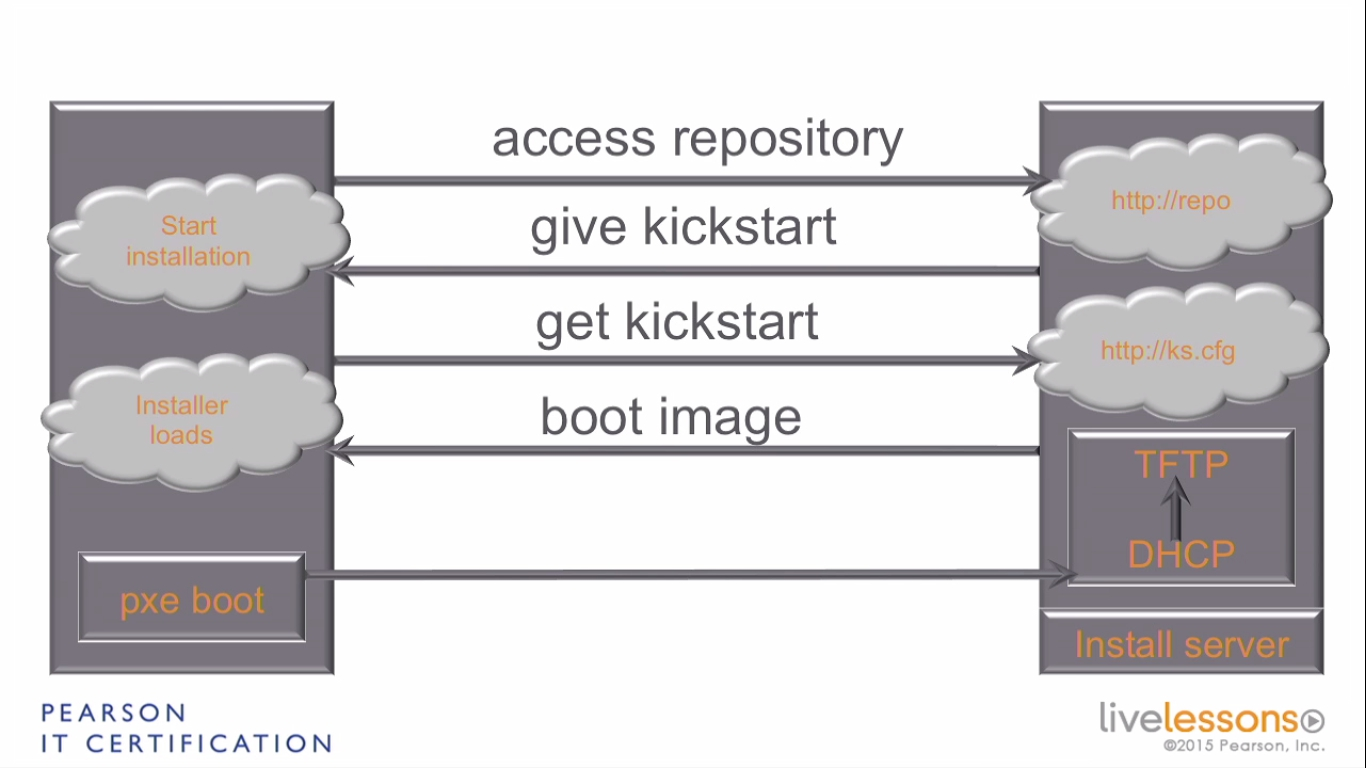
\includegraphics[width=0.9\linewidth]{RHCSA/Mod3/chapters/3.18.a}
	\caption{PXE (Network) boot with Kickstart}
	\label{fig:3 Network boot with Kickstart}
\end{figure}

\noindent
However, since here the OS is installed using a Kickstart file, the client sends a request to receive a copy of the kickstart file from the web/FTP server on the installation server. Upon receiving the kickstart file, finally the installation begins. Finally, the installation needs access to the repository on the installation server for the rpm files that the installer will install (since the installation server is also the installation source). The repository needs to be pre-configured on the installation server as well. 